%
% common information to the web version and print version
%
% images will be imported by searching the paths set with \graphicspath
% the book.tex or web.tex sets this so the correct resolution images end
% up in the correct document.
% 

% title page

{\huge This boy is from Steppe}
% front cover for web version
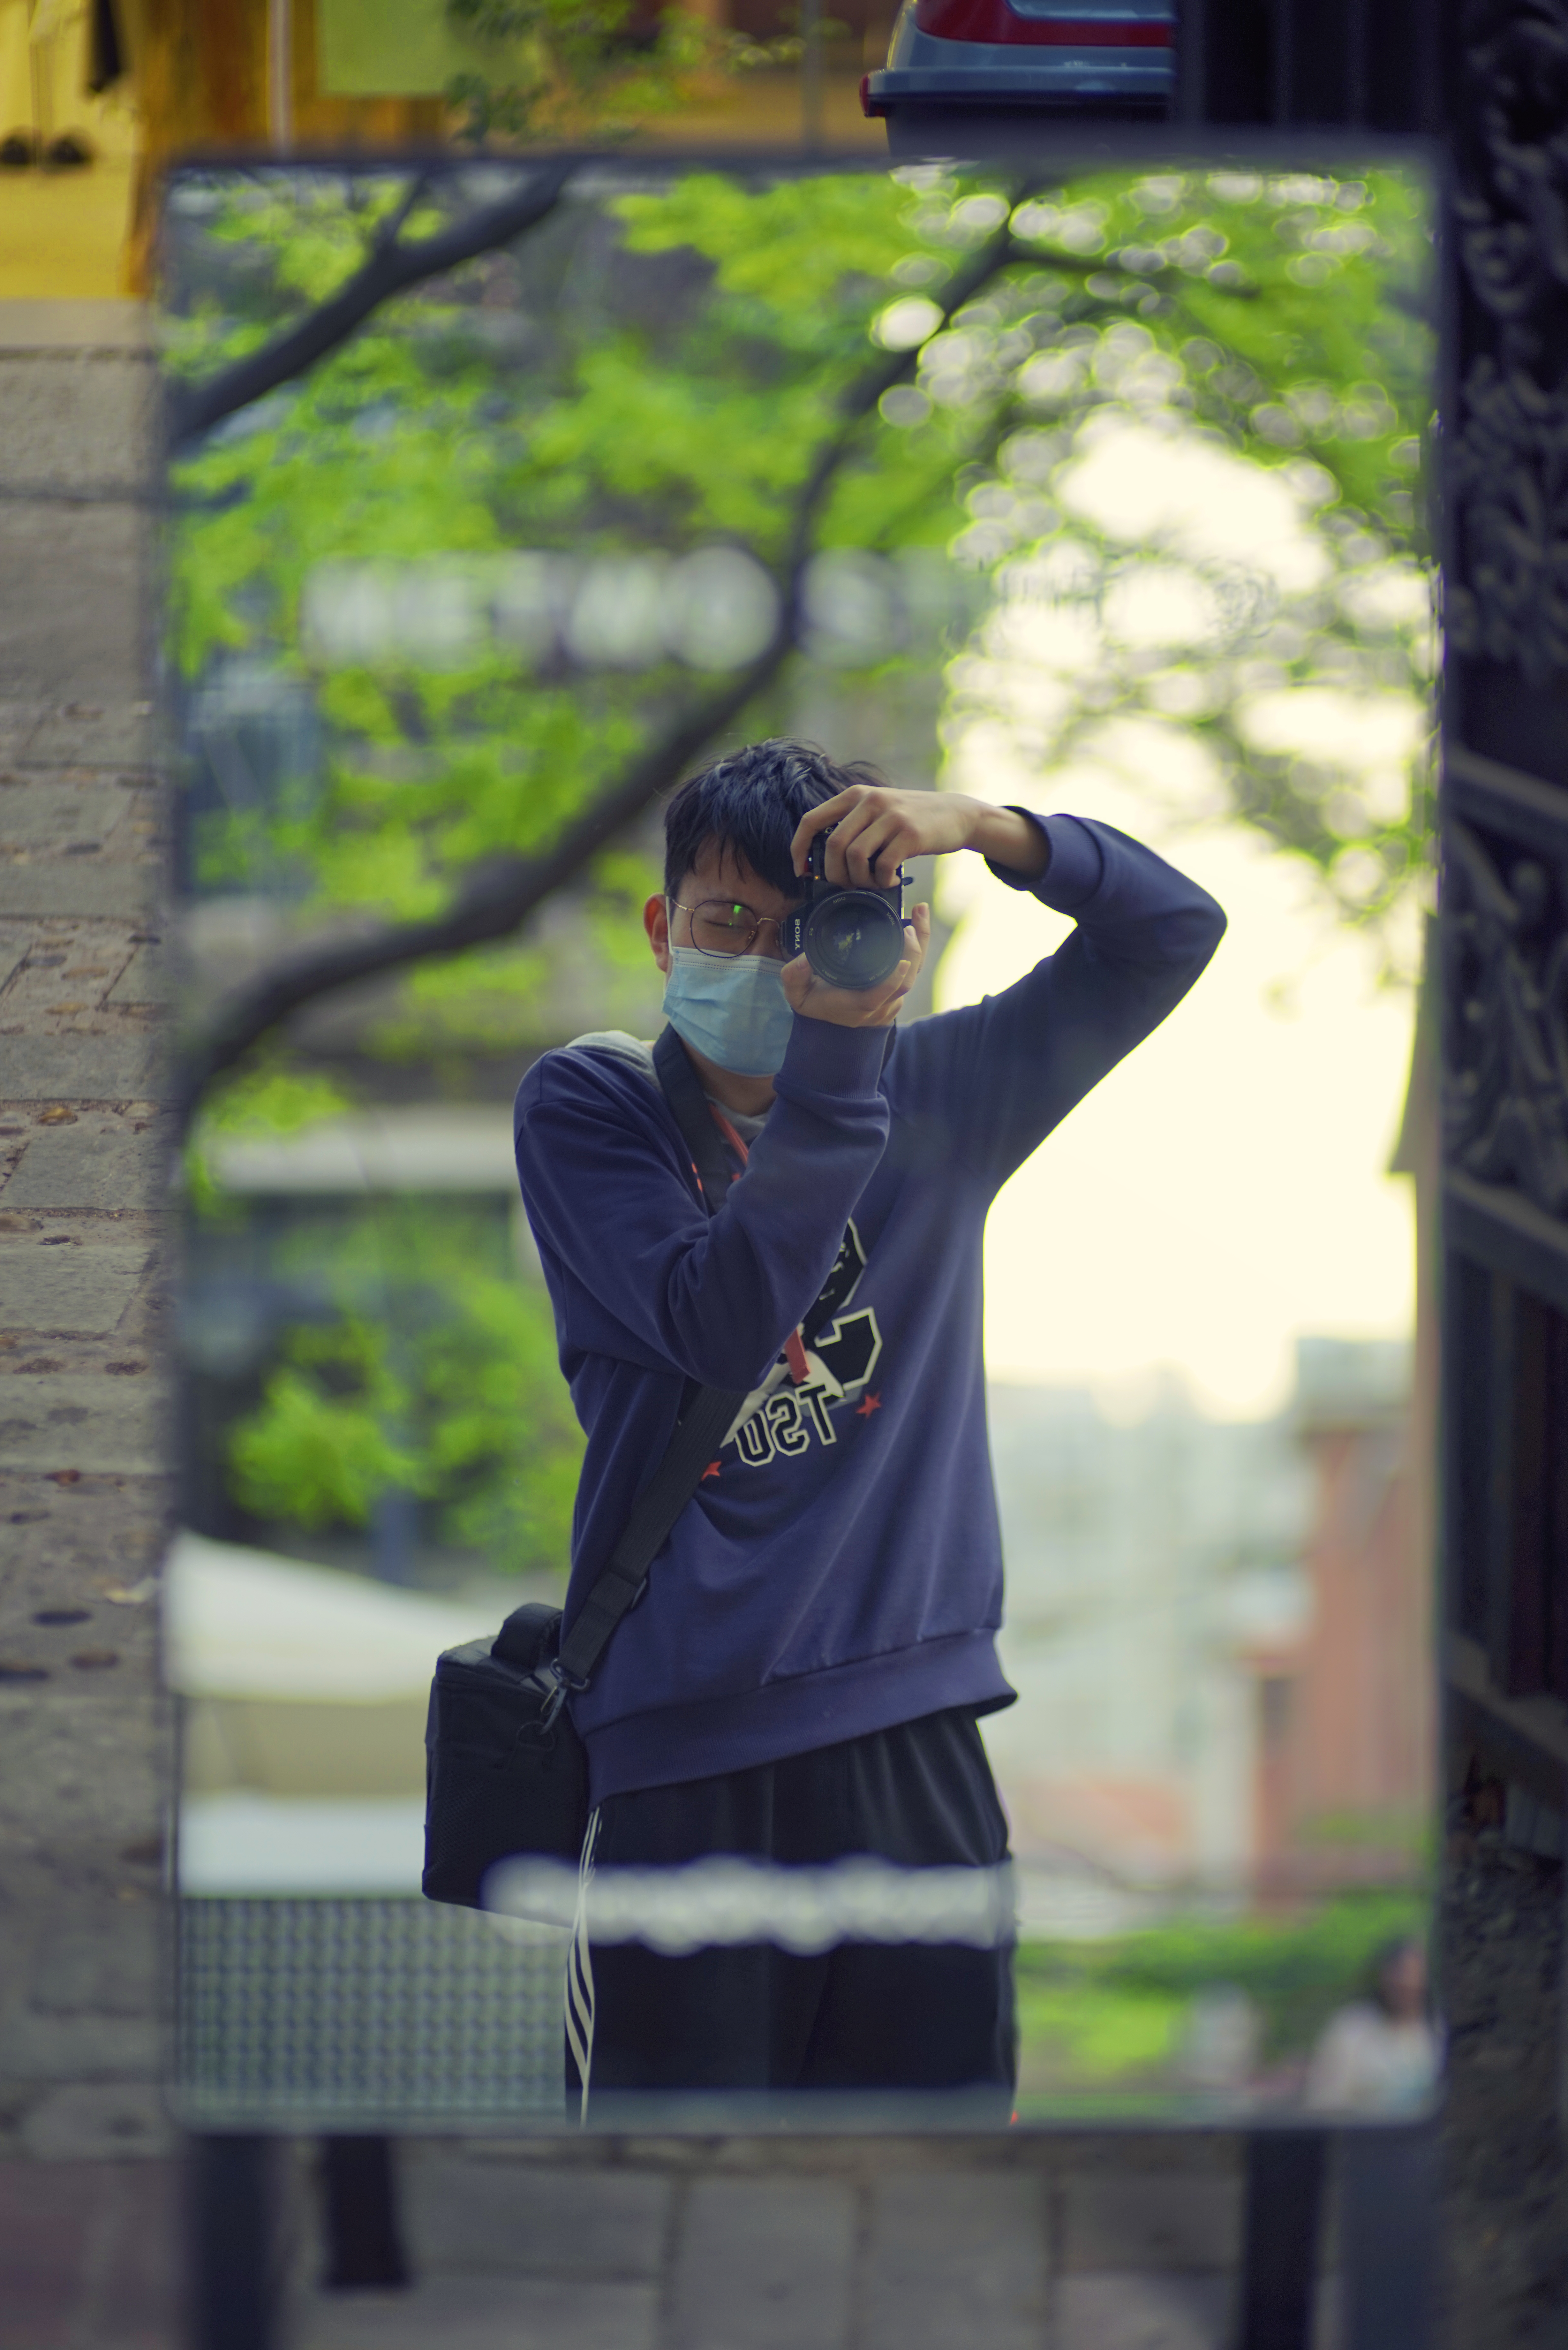
\includegraphics[width=4in]{me.jpg}

\begin{flushright}
{\Large by Lu Tao}
\end{flushright}
\newpage

% front matter page

\vspace*{1in}
{\LARGE About}
\vspace*{0.25in}

He's speed most of my childhood in Hohhot, Inner Mongolia. 
The scene of the steppe in my hometown keeps flashing back in his mind these days.  
And it inspires he to make this album in memory of my past days.
These photographs represent some part of him.
To some extent, to read this book is to read about this boy.

\vspace*{1.0in}

{\large Copyright \copyright \  2009 Eric R. Jeschke.  All Rights Reserved.}

This folio may not be reproduced in any form without written permission
of the author. 

{\tt eric@redskiesatnight.com}

\newpage

% here come the images, one per page
{ 
\pagecolor{photopagecol}

\kphoto[width=8in,height=6in]{R20090606-093158}{}
\newpage

\kphoto[width=8in]{R20090619-101312-curves}{}
\newpage

\kphoto[width=8in]{R20090619-101502-levels}{}
\newpage

\kphoto[width=8in]{R20090619-101707-curves}{}
\newpage

\kphoto[width=8in]{R20090619-101832-levels}{}
\newpage

\kphoto[width=8in]{R20090619-101948}{}
\newpage

\kphoto[width=8in]{R20090619-102238}{}
\newpage

\kphoto[width=8in]{R20090619-102446-curves}{}
\newpage

\kphoto[width=8in]{R20090619-102632-levels}{}
\newpage

\kphoto[width=8in]{R20090606-151823}{}
\newpage

\kphoto[width=8in]{R20090619-103748}{}
\newpage
}

\pagecolor{textpagecol}
\vspace*{1in}

{\LARGE Colophon}
\vspace*{0.25in}

Eric Jeschke finds life with a camera more fulfilling.
You can see more of Eric's photography at

\url{http://redskiesatnight.com/}

For more information about the book, {\em Chickens, Anyone?}, visit

\url{http://redskiesatnight.com/books/chickens-anyone}

\vspace*{0.25in}

This folio was created using \LaTeX and {\em xelatex}.
The font used is Garamond.

\vspace*{0.5in}

\begin{center}
\includegraphics[width=1.5in]{R20080416-135900}
\end{center}

%END
